%%% Time-stamp: <mainrep.tex 19:57, 17 Jul 2016 by P Sunthar>
%%% $Log:$
% This document describes how to use iitbreport style
%********************************************************************

%\documentclass[11pt,a4paper,openright]{report}
\documentclass[twoside]{iitbreport}

%% Default spacing: 1.5
%% Default font size: 12pt
%% Default font: txfonts (similar to times new roman)

%% Selectively comment out sections that you want to be left out but
%% maintaining the page numbers and other \ref
\includeonly{%
  intro/introduction,
  lit/literature,
  expt/experimental,
  rnd/results,
  dem/dem,
  sph/sph,
  coupling/coupling,
  dec,abs,pub,ack
}

%%% Some commonly used packages (make sure your LaTeX installation
%%% contains these packages, if not ask your senior to help installing
%%% the packages)

\usepackage{booktabs}
\usepackage{graphicx}
\usepackage{amsmath}
\usepackage{hyperref}
\usepackage{caption}
\usepackage{subcaption}
\usepackage[T1]{fontenc}
\usepackage{lmodern}
\graphicspath{{expt/}}


%%% Macro definitions for Commonly used symbols
\newcommand{\Rey}{\ensuremath{\mathrm{Re}}}
\newcommand{\avg}[1]{\ensuremath{\overline{#1}}}
\newcommand{\tenpow}[1]{\ensuremath{\times 10^{#1}}}
\newcommand{\pder}[2]{\ensuremath{\frac{\partial#1}{\partial#2}}}

% Referencing macros
\newcommand{\Eqref}[1]{Equation~\eqref{#1}}
\newcommand{\Tabref}[1]{Table~\ref{#1}}
\newcommand{\Figref}[1]{Figure~\ref{#1}}
\newcommand{\Appref}[1]{Appendix~\ref{#1}}


\begin{document}

%%********************************Frontmatter***********************
% In frontmatter everything comes with roman numbering
\pagenumbering{roman}
\setcounter{page}{1}

%*******************************************************************
%                         Title Page
%*******************************************************************
\title{Smoothed Particle Hydrodynamics-Discrete Element Method Coupling}
\author{Dinesh A}

%% Print the date. Today's date comes by default, change it here to
%% other date format, if required:

%\date{\today}
%\date{10 Mar 2016}


%% The type of the report can be set here

% \reporttype{A Seminar Report}
\reporttype{A Thesis}
%\reporttype{A Dissertation}
%\reporttype{A Project Report}

%% Name of the degree
% \degree{Doctor of Philosophy}
\degree{Master of Technology}


%% Department/Centre Name
\dept{Department of Aerospace Engineering}

%% Supervisor and cosupervisor/excosupervisor are not essential parts
%% of a report title page, as it is your report!

%% But if you **have** to put it uncomment these
%\supervisor{Supervisor name}
%\cosupervisor{Co-super name}
%\excosupervisor{External Supervisor}

%% Roll number
\rollnum{Roll No. 153010009}

\maketitle

%*******************************************************************
%                         Copyright Page
%*******************************************************************
%\mycopyright

%*******************************************************************
%                         Dedication Page
%*******************************************************************
\dedication[Dedicated to \ldots]
%\addintoc{Dedication}

%*******************************************************************
%                        Certificate Page
%*******************************************************************
%\makecertificate[change title name]{report type}
\makecertificate{seminar report}
%\makecertificate{thesis}
%\makecertificate{dissertation}
%\makecertificate{project report}

%\addintoc{Certificate}

%*******************************************************************
%                         Approval Sheet
%*******************************************************************
%\makeapproval{thesis}
%\makeapproval{dissertation}

%*******************************************************************
%                          Declaration
%*******************************************************************
%==================================dec.tex================================
%
\begin{Declaration}
\noindent
I declare that this written submission represents my ideas in my own words and where others' ideas or words have been included, I have adequately cited and referenced the original sources. I declare that I have properly and accurately acknowledged all sources used in the production of this report. I also declare that I have adhered to all principles of academic honesty and integrity and have not misrepresented or fabricated or falsified any idea/data/fact/source in my submission. I understand that any violation of the above will be a cause for disciplinary action by the Institute and can also evoke penal action from the sources which have thus not been properly cited or from whom proper permission has not been taken when needed.

%
%
%
%
%
%
%

\DecSign[\today]



%
\end{Declaration}
%========================================================================

















%\addintoc{Declaration}

%******************************************************************
%                          Abstract
%******************************************************************
%============================= abs.tex================================
\begin{Abstract}
This document contains essential templates required to write technical
reports using \LaTeX.  Particularly it shows how to create an
equation, figure, table, symbols list, and bibliographic citation in a \LaTeX\
document.
%
%
%
%
%
\end{Abstract}
%=======================================================================



%******************************************************************
%                         Contents list
%******************************************************************
%\figurespagefalse
%\tablespagefalse
\makecontents % Creats toc, lof, and lot

%******************************************************************
%                        Notations
%******************************************************************
\notations[4cm]{List of Symbols}

%%********************************Mainmatter***********************
% In mainmatter everything comes with arabic numbering
\cleardoublepage
\setcounter{page}{1}
\pagenumbering{arabic}

%******************************************************************
%                         Chapters
%******************************************************************

\newcommand{\etas}{\ensuremath{\eta_{\mathrm{s}}}}


\chapter{Introduction}


This document contains commonly used essential templates to write a
\LaTeX\ document. This document is to be used along with the files and
folders provided. Writing a \LaTeX\ document is very simple.  Often
students need only very simple constructs.  This document shows
certain essential features that almost all technical report writing
requires. Please consult the PDF file for the output of the document,
and then look at the corresponding \LaTeX\ file to reproduce it.  The
document illustrates the following constructs
\begin{itemize}
\item Unnumbered and numbered Lists
\item Equations
\item Defining short macros for frequently used symbols
\item Bibliography
\item Figures
\item Tables
\end{itemize}

The normal procedure for compiling a \LaTeX\ document that contains
bibliographic entries is to follow the following steps
\begin{enumerate}
\item \verb|pdflatex mainrep|
\item \verb|bibtex mainrep|
\item \verb|pdflatex mainrep|
\item \verb|pdflatex mainrep|
\end{enumerate}
In the above example \verb|mainrep| is the main \LaTeX\ file.


\section{First section of this chapter}

This is the first chapter, which resides in a directory (folder)
intro. Each chapter can contain \verb|section|, \verb|subsection|
and so on.

\subsection{Equations and Math symbols}


Equations should be set in a separate mode.  For details on getting
various types of aligned equations, consult the \AmS-\LaTeX\
documentation \verb|amsldoc.pdf|. Simple equations are set as
\begin{equation}
\label{eq:sinx}
\int \mathrm{d}x \; \cos x =  \sin x
\end{equation}
Equation~\eqref{eq:sinx} is the integral of the cosine
function. Mathematical symbols must always be put inside \verb|$$|,
when they appear outside a math environment (such as \verb|equation|,
\verb|align|, \verb|gather|, etc).  The symbol ``ex'' must be written as
$x$ and not as x.  

Another commonly used construct for equations is the \verb|align|
environment to align several equations along a vertical line. It is
usually the $=$ sign across which the alignment is done.  The
point of alignment for each equation is specified using the ampersand symbol 
\begin{align}
a &= b  \\
a + e + f + g & = m + n + z \\
x + 2 & = x^{3} + 3 x^{2} + 2 x + 5
\end{align}

\subsection{Commonly used Symbols}
For mathematical symbols it is very convenient to define frequently
used symbols as a short macro. For example if you are to be using the
symbol $\eta_{\mathrm{s}}$ frequently it is convenient to define it in
as:\\
\verb|\newcommand{\etas}{\ensuremath{\eta_{\mathrm{s}}}}| \\
in the preamble and to simply refer it to in the text as \etas\ or in
a mathematical equation as $\etas = \eta \, ( 1 + \phi)$.
%%
%

\section{How to write nomenclature} 

\subsection{General guidelines:}
\begin{enumerate}	
	\item Use \verb|\nomenclature[prefix]{symbol}{description}| for symbols, the best place for this command is immediately after you introduce the symbol for the first time
	\item Shorten the long command:\\ \verb|\newcommand{\nm}[2]{\nomenclature{#1}{#2}}|
	\item Create compiler for nomenclature with the given code: \\
	\textbf{makeindex \%.nlo -s nomencl.ist -o \%.nls -t \%.nlg }\\
	For TeXstudio: go to options > build > user command > write- `user1: Nomenclature' amd paste the above code\\
	For compiling the nomenclature: go to tools > user > Nomenclature	
\end{enumerate}	

\subsection{Grouped nomenclature}
\begin{enumerate}
\item For acronyms, use:\\
 \verb|\nmA[sorting letter]{symbol}{descritpon}|
\item For roman symbols, use:\\
\verb|\nmR[sorting letter]{symbol}{descritpon}|
\item For greek symbols, use:\\
 \verb|\nmG[sorting letter]{symbol}{descritpon}|
 \item For superscripts, use:\\
 \verb|\nmS[sorting letter]{symbol}{descritpon}|
 \item For subscripts, use:\\
 \verb|\nms[sorting letter]{symbol}{descritpon}| 
 \item For any other symbol, use:\\
 \verb|\nmX[sorting letter]{symbol}{descritpon}|\\
 Name of other symbols can be changed with \verb|\OtherSym{Name of symbols}|
\end{enumerate}
%%
\subsection{Some examples}
\begin{enumerate}
\item \verb|\nmA[FF]{FFA}{Free fatty acid}|
\item \verb|\nmA[AO]{AOR}{Angle of repose}|
\item \verb|\nmR[Ra]{$R$}{Radius of circle}|
\item \verb|\nmR[ra]{$r$}{Intrinsic length}|
\item \verb|\nmR[Gr]{$G_\mathrm{r}$}{Gravity}|
\item \verb|\nmG[al]{$\alpha_{\mathrm{a}}$}{Angular acceleration}|
\item \verb|\nmG[et]{$\eta$}{Viscosity}|
\item \verb|\nmG[be]{$\beta$}{Shape factor}|
\item \verb|\nmS[v]{$v$}{Vapor phase}|
\item \verb|\nmS[g]{$g$}{Gas phase}|
\item \verb|\nms[i]{$i$}{Indices}|
\item \verb|\nms[x]{$x$}{Variable in x-direction}|
\item \verb|\nmX[f]{foo}{foo|
\end{enumerate} 

\nmA[FF]{FFA}{Free fatty acid}
\nmA[AO]{AOR}{Angle of repose}


\nmR[Ra]{$R$}{Radius of circle}
\nmR[ra]{$r$}{Intrinsic length}
%\nmR[Gr]{$G_\mathrm{r}$}{Gravity}


\nmG[al]{$\alpha_{\mathrm{a}}$}{Angular acceleration}
\nmG[et]{$\eta$}{Viscosity}
%\nmG[be]{$\beta$}{Shape factor}


\nmS[v]{$v$}{Vapor phase}
\nmS[g]{$g$}{Gas phase}


\nms[i]{$i$}{Indices}
\nms[x]{$x$}{Variable in x-direction}


\nmX[f]{foo}{foo}


%%


%%% Local Variables: 
%%% mode: latex
%%% TeX-master: "../mainrep"
%%% End: 


\chapter{Literature Survey}

The bibliographic entries are to be kept in a file named
\verb|<something>.bib|. In this sample report we call it as
\verb|mylit.bib|. This file must be included without the \verb|.bib|
extension in the main file as: \verb|\bibliography{mylit}|.   Open the
file \verb|mylit.bib| to see the format in which the entries are
written. This is written in the Bib\TeX format. Most of the
bibliographic web pages (Scopus, ISI Web) and software (EndNote, etc)
allow you to export bibliographic entries in the Bib\TeX format.

Citations are referred in the text using \verb|\citet| command which produces citations as though they are part of the text.  In order to say
somebody did this work as a part of a line use:
\verb|\citet{Batzri1973}| have done extensive work on \ldots.  This will produce
\citet{Batzri1973} have done extensive work on \ldots. Alternately citations can appear in parenthesis.  
The command~\verb|\citep{Batzri1973}| is used to automatically put the
citations in parenthesis.  As an example consider the extensive work
done in the area of book writing \citep{Sackmann1995a,Boal2012}.

Conferences \citep{rich-mart92} or collection of work
\citep{Sackmann1995a} also have special entries.

It is also possible to cite thesis like this:
\citet{jariwala00,luding94} or just unpublished work from
\citet{SunHI03}. Some times there are unclassified bibliographic
entries which can be put under ``misc'' \citep{Smith99}.



%%% Local Variables: 
%%% mode: latex
%%% TeX-master: "../mainrep"
%%% End: 


\chapter{Materials and Methods}

\section{Including Figures}

Figures are conveniently included using postscript format.  If you are
generating a figure in a software, please check if the software
supports writing to a postscript or a PDF format. This format is loss
less vector format and with reproduce in any magnification without any
pixelation. Make sure to write it to an ``Encapsulated Post-script''or
.eps format.


\begin{figure}[tbp]
  \centering
    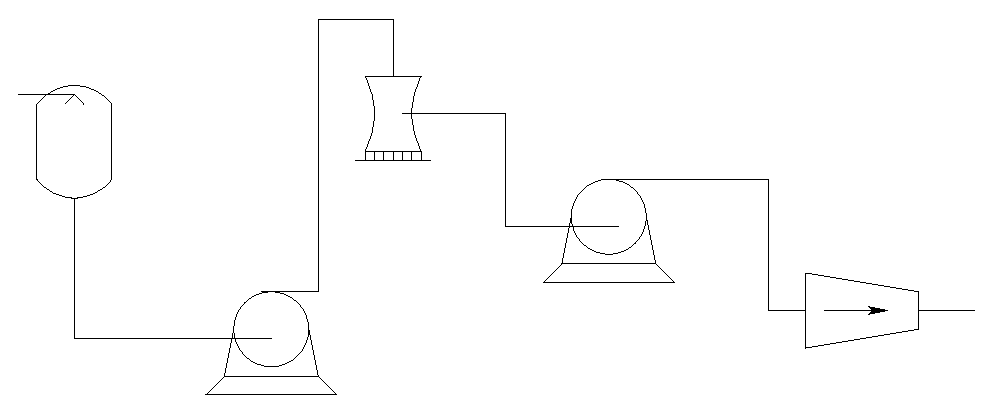
\includegraphics[width=0.7\textwidth]{profflow}
    \caption[Process flow sheet]{Process flow sheet of the
      experimental setup. The caption of the figure goes here. A
      shorter caption can be written in square brackets to identify it
      in the list of figures.}
    \label{fig:pfs} 
\end{figure}

Figures should be given a label and which can be used to refer to them
in the running text using \verb|\ref{}| command. Figure~\ref{fig:pfs}
describes the process flow sheet of the experimental set up used in
this report. The \Figref{fig:pfs} can also be refered by a short form notation
a pre-defined macro \verb"\Figref".



%%% Local Variables: 
%%% mode: latex
%%% TeX-master: "../mainrep"
%%% End: 

\chapter{Results and Discussions}


\section{Discrete element method}

As a first benchmark, studying a freely falling solid sphere onto a
floor. Solid sphere has radius $r_p = 10$ cm, density $\rho_p$ = 2.6 *
1e3 $kg/m^3$, falls from a height $h_0 =$ 0.5 m under gravity.


For a freely falling solid, we have an analytical solution. Implementing
it using DEM, and comparing the results could give us an idea of accuracy of
the numerical method. Here we compare analytical solution of  position and velocity
with DEM result.



\section{Smoothed Particle Hydrodynamics}


\section{SPH DEM coupling}

%%% Local Variables:
%%% mode: latex
%%% TeX-master: "../mainrep"
%%% End:

\chapter{Discrete Element Method}

It is a numerical method introduced by Cundall and Strack \citep{CS79}
used to model the behaviour of large number of particles having finite
mass and radius which interact at their surfaces. The governing
equation of motion for such a particle can be written using Newton's
laws.

\begin{align}
  \label{eq:newton_equation_of_motion}
  \frac{d^2 \vec{x}}{dt^2} = \vec{F}(\vec{x}, \vec{v}, m)\\
  \frac{d^2 \vec{\omega}}{dt^2} = \vec{M}(\vec{x}, \vec{v}, m)
\end{align}

Where $\vec{F}$, $\vec{M}$ is the force and moment acting on the
particle. m, $\vec{v}$, $\vec{x}$ are the mass, position and velocity
of the particle.
The force $\vec{F}$ in equation\ref{eq:newton_equation_of_motion} is
the one to be computed during each time step. This force arises due to
collision of particles.

% \begin{figure}
%   \centering
%   \includegraphics[scale=0.5]{dem/two_pars_in_contact}
%   \caption{Two spherical particles in contact}
%   \label{fig:tspc}
% \end{figure}

Before studying the interaction of a particle with wall or any other
spherical particle, lets consider a spherical particle with mass m
freely falling under gravity. For such a model, the governing
differential equation can be written as

\begin{align}
  \label{eq:free_fall}
  \frac{d^2 \vec{x}}{dt^2} = \vec{g}\\
  \frac{d^2 \vec{\omega}}{dt^2} = 0
\end{align}

Such a differential equation \eqref{eq:free_fall} governs a scene like
in figure \eqref{fig:free_fall}

\begin{figure}
\centering
\begin{subfigure}{.5\textwidth}
  \centering
  \includegraphics[scale=0.3]{dem/free_fall}
  \caption{A freely falling Sphere}
  \label{fig:free_fall}
\end{subfigure}%
\begin{subfigure}{.5\textwidth}
  \centering
  \includegraphics[scale=0.3]{dem/bounce_back}
  \caption{A freely falling Sphere onto a wall}
  \label{fig:bounce_back}
\end{subfigure}
\caption{Behaviour of sphere under different conditions}
\label{fig:sphere_intro}
\end{figure}


In freely falling situation, the particle doesn't see any obstacles,
and follows a straight line path.

Now assume that there is a wall obstructing the motion of this
spherical ball.  As the ball hits the wall it has to bounce back
\eqref{fig:bounce_back}, because of the repulsion force from the
wall. There are two ways to model such a behaviour.

\begin{itemize}
\item Event driven method (hard particles)
\item Discrete element methods (soft particles)
\end{itemize}


Present work deals with Discrete element method, with a little introduction
to Event driven method.

\section{Discrete element method (DEM)}
\label{sec:edm}

In this method at every instant of time the ball is checked if it is
in contact with any other particle or wall. If it is, then the force
is computed from the relative positions of the overlapping
particles. By using such force($\vec{F}$) \eqref{eq:newton_equation_of_motion} is
integrated using Euler or RK2.

\subsection{Force calculation}
\label{sec:force}

\begin{figure}
  \centering
  \includegraphics[scale=0.5]{dem/collision}
  \caption{Two spherical particles in contact}
  \label{fig:tspc}
\end{figure}

\begin{equation}
  \label{eq:overlap}
  \delta = (r_i + r_j) - |\vec{X}_{i} - \vec{X}_{j}|
\end{equation}

Say two particles \eqref{fig:tspc} i and j with radii $r_{i}$ and
$r_{j}$, are in contact if $\delta$ \eqref{eq:overlap} is positive.
The particle i has linear velocity $\vec{V}_{i}$ and angular velocity
of $\vec{\omega}_{i}$ particle j has linear velocity $\vec{V}_{j}$ angular
velocity of $\vec{\omega}_{j}$.

The unit normal vector along particle i to particle j  is given by

\begin{equation}
  \label{eq:normal_unit}
  \vec{n}_{ij} = \frac{\vec{X}_{j} - \vec{X}_{i}}{|\vec{X}_{j} - \vec{X}_{i}|}
\end{equation}

The relative velocity of point of contact becomes

\begin{equation}
  \label{eq:relative}
  \vec{V}_{ij} = \vec{V}_{i} - \vec{V}_{j} +
  (r_{i} \vec{\omega}_{i} + r_{j} \vec{\omega}_{j}) \times \vec{n}_{ij}
\end{equation}

Therefore the normal and tangential components of contact velocity are

\begin{equation}
  \label{eq:normal_vel}
  \vec{V}_{nij} = \vec{V}_{ij} \cdot \vec{n}_{ij} \vec{n}_{ij}
\end{equation}

\begin{equation}
  \label{eq:tang_vel}
  \vec{V}_{tij} = \vec{V}_{ij} - \vec{V}_{ij} \cdot \vec{n}_{ij} \vec{n}_{ij}
\end{equation}

The tangent to the plane of contact is

\begin{equation}
  \label{eq:tang_unit}
  \vec{t}_{ij} = \frac{\vec{V}_{tij}}{|\vec{V}_{tij}|}
\end{equation}


Discrete element method is a soft sphere approach. In soft sphere
approach the overlap between two particles is described by a spring
and a dashpot in both normal and tangential direction. Generally, when
two particles collide, there will be a repulsion force on both the
particles. This repulsive force is represented by springs, whose
magnitude depends on the overlap amount. Similarly, when a collision
occurs, there will be damping of energy due to deformation of the body
and the friction force between the particles. This damping is
introduced by the dashpot between the particles. The respective spring
and damping coefficients depend on the coefficient of restitution
between the colliding particles and the material properties of the
colliding particles.



%%


%%% Local Variables:
%%% mode: latex
%%% TeX-master: "../mainrep"
%%% End:

\chapter{Smoothed Particle Hydrodynamics}
\label{chap:SPH}

In the present work Smoothed Particle Hydrodynamics (SPH), a particle based
framework is used to study the fluid motion, using Navier-stokes
equation as basis for fluid motion.


\section{Introduction to SPH}


It is invented by \cite{lucy1977numerical} and
\cite{gingold1977smoothed} independently to model astrophysical
simulations. The basic idea of SPH is representing a field variable
A from known values of A through interpolation integrals in the given
domain. This could be written in terms of Dirac delta function as follows

\begin{equation}
  \label{eq:dirac_repr}
  A(\boldsymbol{x}) = \int_{\Omega}\> A(\boldsymbol{x}') \> \delta(\boldsymbol{x} - \boldsymbol{x}') \> d\boldsymbol{x}'
\end{equation}

Where x is the point of interest in the domain, $\omega$ is volume of
the domain and $d\boldsymbol{x}'$ is the differential volume element.
To prove that the above equation \eqref{eq:dirac_repr} interpolates the
field variable correctly, since Dirac delta function is zero except at
$\boldsymbol{x}$, and at $\boldsymbol{x}$ A is constant, so one can take
A out of the integral, which gives us the value at $\boldsymbol{x}$.


\begin{align*}
  \label{eq:dirac_derivation}
  A(\boldsymbol{x}) &= \int_{\Omega}\> A(\boldsymbol{x}') \> \delta(\boldsymbol{x} - \boldsymbol{x}') \> d\boldsymbol{x}'\\
  A(\boldsymbol{x}) &= A(\boldsymbol{x}) \int_{\Omega}\> \> \delta(\boldsymbol{x} - \boldsymbol{x}') \> d\boldsymbol{x}'\\
  A(\boldsymbol{x}) &= A(\boldsymbol{x}) \\
\end{align*}

A can be approximated by replacing the delta function with a smoothing
kernel W, with smoothing length h. Resulting interpolation equation is given by

\begin{equation}
  \label{eq:kernel_repr}
  A(\boldsymbol{x}) = \int_{\Omega}\> A(\boldsymbol{x}') \> W(\boldsymbol{x} - \boldsymbol{x}', h)  \> d\boldsymbol{x}'
\end{equation}

The smoothing function W is usually chosen to be as even function
satisfying few properties.

The first condition is Unity condition:

\begin{equation}
  \label{eq:unity}
  \int_{\Omega}\> W(\boldsymbol{x} - \boldsymbol{x}', h)  \> d\boldsymbol{x}' = 1
\end{equation}

The second condition is kernel function W behaving like delta function
as the influence length h goes to 0. Since delta function has infinite
value at a single point and zero at rest, similarly when the influence
length of the kernel function goes to zero, it should behave like
delta function.

\begin{equation}
  \label{eq:kernel_delta}
  \lim_{h \to 0} W(\boldsymbol{x} - \boldsymbol{x}', h) = \delta(\boldsymbol{x} - \boldsymbol{x}', h)
\end{equation}

And the third condition is having a compact support. As discussed before
that the kernel function has a support, and out of that support the value of
it has to be zero. It is given by \eqref{eq:compact_support}

\begin{equation}
  \label{eq:compact_support}
  W(\boldsymbol{x} - \boldsymbol{x}', h) = 0 \>\>\>\>    when  \>\>\> |\boldsymbol{x} - \boldsymbol{x}'| > kh
\end{equation}

Where k depends on the smoothing kernel chosen.

Changing continuous form of \eqref{eq:kernel_repr} to particle form using
the particles in the domain of interest.

Assume that the domain is discretized into N particles with mass $m_i$ and volume
$dv_i$. We have

\begin{equation}
  \label{eq:mass_repr}
  m_j = dv_i \> \rho_i
\end{equation}

Using \eqref{eq:mass_repr}, \eqref{eq:kernel_repr} is converted to
discrete form as follows

\begin{equation}
  \label{eq:discrete_form}
  A_i = \sum\> \frac{m_j}{\rho_j} A_j\> W(\boldsymbol{x}_i - \boldsymbol{x}_j, h)
\end{equation}

Where $A_i$ is the value of the field property of particle i,
similarly for $A_j$.

Similarly derivative of a field variable can be written as

\begin{equation}
  \label{eq:discrete_derivative}
  A_i = \sum\> \frac{m_j}{\rho_j} A_j\> \nabla W(\boldsymbol{x}_i - \boldsymbol{x}_j, h)
\end{equation}


\section{Fluid equations of motion}

Navier-Stokes equations are a set of partial differential equations
that are used to describe the motion of fluids. These equations are
used to model different types of scenarios like : air flow through
cars, aeroplanes, and etcetera.  For fluid phase the following
equations are used.

The equation of motion is given by


\begin{equation}
  \label{eq:momentum_eq}
  \rho \>\frac{d\textbf{v}}{dt} = - \nabla p + \mu\> \nabla^2\textbf{v} + \textbf{f}
\end{equation}

Where \textbf{v} is flow velocity, $\rho$ is density, p is the
pressure and \textbf{f} is body force. In order to compute the right
hand side of \eqref{eq:momentum_eq} we need information, such as
density of the fluid, and pressure at every time step, which could be
obtained using other equations.


In Lagrangian point of view  \eqref{eq:momentum_eq} is written as

\begin{equation}
  \label{eq:momentum_eq}
  \rho \>\frac{\partial\textbf{v}}{\partial t} = - \nabla p + \mu\> \nabla^2\textbf{v} + \textbf{f}
\end{equation}

This could be written in terms of forces acting on a particle with mass m as

\begin{equation*}
  \label{eq:forces_eq}
  m_i \>\frac{\partial\textbf{v}_i}{\partial t} = -V_i \nabla p_i + V_i \mu\> \nabla^2\textbf{v} + V_i \textbf{f}
\end{equation*}

The right hand side of \eqref{eq:forces_eq} are the forces acting on
particle i due to pressure of neighbouring particles, shear force due
to relative motion between neighbouring particles, and the third term
is the body force. Here there is a clear advantage of particle approach,
suppose in future if one has to apply surface tension between particles,
or force due to solid body immersed in fluid, or due to porous media,
one could simply add the force term to this equation \eqref{eq:forces_eq}.


After computing the forces on each particle, respective accelerations are calculated
from the following

\begin{equation*}
  \label{eq:total_force}
    \textbf{F}_i = \textbf{F}_{i}^{Pressure} + \textbf{F}_{i}^{viscous} + \textbf{F}_{i}^{additional}
\end{equation*}

\begin{equation}
  \label{eq:acceleration}
    \textbf{a}_i = \frac{\textbf{F}_i}{m_i}
\end{equation}

By using appropriate integration schemes like RK2, Euler, Prediction
correction algorithms the system is moved forward by computing
velocity and position of the particles at every time step by using
acceleration computed from \eqref{eq:acceleration}


As discussed previously in order to compute the pressure force we need
additional equations to solve for pressure computations. Since in the
present work we deal with WCSPH, pressure is directly related to
density with Tait equation. From this one could infer that we need to
solve for density at every time step. There are several ways to
compute density in SPH, two methods are discussed in the next section.


\section{Density computation}
\label{sec:density_comp}

Density of a fluid particle in SPH can be computed using many approaches, like

\begin{itemize}
\item Summation density
\item Continuity equation
\end{itemize}

SPH way of density computing is using summation density. It is derived from basic
function interpolation in SPH. It could be derived as follows.

From \eqref{eq:summation_mass_rep} we have,

\begin{equation*}
  \label{eq:summation_mass_rep}
  A_i = \sum\> \frac{m_j}{\rho_j} A_j\> W(i,j)
\end{equation*}

Where, $A_i$ is the property we are interested in. Here it is density,
by substituting $A_i$ with $\rho_i$ we have

\begin{align}
  \label{eq:summation_mass_rep}
    \rho_i &= \sum\> \frac{m_j}{\rho_j} \rho_j\> W(i,j) \nonumber \\
    \rho_i &= \sum\> m_j \> W(i,j)
\end{align}


By using \eqref{eq:summation_mass_rep} one gets lower density values
at the free surface of the fluid. This is due to lack of particle
support. In order to prevent such thing, Shepard filter is applied.

In the second approach from continuity equation the rate of change of
density is calculated, through which the density at a time is
computed.

\begin{align}
  \label{eq:continuity}
    \frac{d\rho}{dt} = -\rho \nabla * \textbf{v}
\end{align}

\eqref{eq:continuity} is discretized in terms of particles and written
in summation form as follows

\begin{align}
  \label{eq:sph_continuity}
    \frac{d\rho_a}{dt} = \sum_{b}m_b \textbf{v}_{ab} * \nabla_a W_{ab}
\end{align}

Once density of the field is calculated, the corresponding pressure is computed using
Tait equations, which is described in next section.


\section{Pressure computation}

Since the fluid is slightly compressible, one can relate pressure with density
of fluid. The reason for considering the fluid to be slightly compressible is because,
if the flow in incompressible, one has to solve for pressure Poisson equation in order to
compute the pressure of the fluid particle, which is quite computationally expensive.
By considering the flow as compressible such time consuming computation could be reduced.

Pressure and density could be related with two equations, they are, the ideal gas equation
and Tait equation. In the present work Tait equation of state is used. Tait equation of
state is given as

\begin{align}
  \label{eq:pressure}
  p_i = \frac{\rho_0 c_s^2 }{\gamma} \bigg(\bigg(\frac{\rho}{\rho_0}\bigg)^\gamma - 1 \bigg)
\end{align}

where c_s is the maximum speed of sound inside the fluid, $\rho_0$ is
the rest density of the fluid and gamma is the polytropic constant.
\eqref{eq:pressure} is extended to handle low density situations as in
free surface flows and near particle leaking. In low density regions
where density of the fluid is less than the fluid density we have
negative pressure which leads to cohesion force rather than repulsive,
which is not entertained. In order to prevent such attraction hg
correction is applied to the equation \eqref{eq:pressure} The corrected
pressure equation is termed to be HG correction.





In SPH, the fluid is discretized into particles, contrast to euerian
grid based scemes. The physical properties of the fluid are obtained
at the particle, where as in eulerian frameworks, the properties are
calcualted at locations.


\section{Smoothing kernels}
\label{sec:sk}


In the present work cubic b-splpine kernel function is used
for averaging the neighbourhood particle contribution. The kernel
function can be written as

\[
  W_{cspline}(r, h) =
  \begin{cases}
    \frac{6 \> r^3}{h^3} - \frac{6 \> r^3}{h^2}, & 0 <= r <= \frac{h}{2}\\
    2 * \big(1 - \frac{r}{h}\big)^3, & \frac{h}{2} <= r <= h\\
    0,                                          & \text{otherwise}
  \end{cases}
\]


\section{Approximating fluid equation of motion with SPH}
\label{sec:fesph}

Navier-Stokes equations are a set of partial differential equations
that are used to describe the motion of fluids. These equations are
used to model different types of scenarios like : air flow through
cars, aeroplanes, and etcetera.  For fluid phase the following
equations are used.

The equatin of motion of a incompressible fluid in lagrangian view
point can be written as

\begin{equation}
  \label{eq:momentum_eq}
  \rho\> \frac{d\textbf{v}}{dt} = -\nabla p + \mu\> \nabla^2\textbf{v} + \textbf{f}
\end{equation}

Multiplying both sides by volume, we get
\begin{equation}
  \label{eq:momentum_eq}
  m\>\frac{d\textbf{v}}{dt} = - V\> \nabla p + V\> \mu\> \nabla^2\textbf{v} + V\> \textbf{f}
\end{equation}

Using SPH the forces on a given particle can be easily computed. Then
these ordinary differential equations can be solved using Euler or RK2
or any other integrating scheme.

\section{Density computation}
\label{sec:density_comp}

Density of a fluid particle in SPH can be computed using many approaches, like

\begin{itemize}
\item Summation density
\item Continuity equation
\end{itemize}

SPH way of density computing is using summation density. It is derived from basic
function interpolation in SPH. It could be derived as follows.

From \eqref{eq:summation_mass_rep} we have,

\begin{equation*}
  \label{eq:summation_mass_rep}
  A_i = \sum\> \frac{m_j}{\rho_j} A_j\> W(i,j)
\end{equation*}

Where, $A_i$ is the property we are interested in. Here it is density,
by substituting $A_i$ with $\rho_i$ we have

\begin{align}
  \label{eq:summation_mass_rep}
    \rho_i &= \sum\> \frac{m_j}{\rho_j} \rho_j\> W(i,j) \nonumber \\
    \rho_i &= \sum\> m_j \> W(i,j)
\end{align}


By using \eqref{eq:summation_mass_rep} one gets lower density values
at the free surface of the fluid. This is due to lack of particle
support. In order to prevent such thing, Shepard filter is applied.

In the second approach from continuity equation the rate of change of
density is calculated, through which the density at a time is
computed.

\begin{align}
  \label{eq:continuity}
    \frac{d\rho}{dt} = -\rho \nabla * \textbf{v}
\end{align}

\eqref{eq:continuity} is discretized in terms of particles and written
in summation form as follows

\begin{align}
  \label{eq:sph_continuity}
    \frac{d\rho_a}{dt} = \sum_{b}m_b \textbf{v}_{ab} * \nabla_a W_{ab}
\end{align}

In the present work WCSPH scheme is used. In WCSPH scheme the flow is
considered to be weakly compressible, which means there could be a variation
in the density of the fluid flow. And the pressure is directly related to density
of the particle by Tait's equation. Once the pressure of each particle is computed, the
resulting forces on a particle due to its neighbours is calculated by the following equation.

\begin{align}
  \label{eq:sph_momentum}
    \frac{d\textbf{v}_a}{dt} = \textbf{g}_a  -\sum_{b}m_b \Bigg(\frac{p_a}{\rho^2_a} + \frac{p_b}{\rho^2_b}\Bigg) \nabla_a W_{ab}
\end{align}

Where $p_a$ is the pressure of the

% Pressure equation:
% ----------------------------------------------
% ----------------------------------------------
% The relationship between pressure and density of a particle is given by

% $$ p_a = B \Bigg[\Bigg(\frac{\rho_a}{\rho_0}\Bigg)^\gamma - 1 \Bigg] $$

% LocalWords:  Tait polytropic Navier eq dirac repr kh discretized dv
% LocalWords:  dt RK WCSPH

\include{coupling/coupling}


%****************************************************************
%                         Appendices
%****************************************************************
%% Additional, supporting material, such as codes, derivations, etc., can be placed in the appendix
\appendix
\chapter{Supporting Material}

%******************************************************************
%                         Bibliography or References
%******************************************************************
\bibliography{mylit}

%*******************************************************************
%                         List of publications
%******************************************************************
%%%
\listofpublications


\noindent Put your publications from the thesis here. The packages \texttt{multibib} or \texttt{bibtopic} or \texttt{biblatex} or enumerate environment or thebibliography environment etc. can be used to handle multiple different bibliographies in the document.








%%======================================================================
%%% Local Variables: 
%%% mode: latex
%%% TeX-master: "../mainrep"
%%% End: 









%*******************************************************************
%                        Acknowledgements
%*******************************************************************
%%%
\acknowledgments

This section is for the acknowledgments. Please keep this brief and resist the temptation of writing flowery prose! Do include all those who helped you, e.g. other faculty/staff you consulted, colleagues who assisted etc.






\signature{\today}
%\signature[Indian Institute of Technology Bombay]{\today}

%========================================================================

%%% Local Variables: 
%%% mode: latex
%%% TeX-master: "../mainrep"
%%% End: 

%*******************************************************************
%                        About author
%*******************************************************************
% \colophon % remove this command while using this file.

% GAME OVER
%*******************************************************************
\end{document}

%%% Local Variables:
%%% mode: latex
%%% TeX-master: t
%%% End:
